\documentclass[12pt]{article}

\usepackage[a4paper,margin=0.5in]{geometry}
\usepackage[square,numbers,sort&compress]{natbib}
\usepackage[utf8]{inputenc} % allow utf-8 input
\usepackage[T1]{fontenc}    % use 8-bit T1 fonts
\usepackage{hyperref}       % hyperlinks
\usepackage{url}            	% simple URL typesetting
\usepackage{booktabs}     % professional-quality tables
\usepackage{amsfonts}     % blackboard math symbols
\usepackage{nicefrac}       % compact symbols for 1/2, etc.
\usepackage{microtype}    % microtypography
\usepackage{amsmath}
\usepackage{algorithm}
\usepackage[noend]{algpseudocode}

\usepackage{graphicx}
\newcommand{\bigo}[1]{{\cal O}\left(#1 \right)}
\newcommand{\p}{\mathrm{P}}
\newcommand{\vect}[1]{\mathbf{#1}}
\newcommand{\indp}[2]{#1 \perp\!\!\!\perp #2}


\begin{document}
\thispagestyle{empty}
\begin{center}

\textbf{DS-GA 1018.001 Probabilistic Time Series Analysis\\
Homework 1}
\end{center}

\noindent \textbf{Due date: Sept. 29, by 6pm}\\
\\
\noindent \textbf{Problem 1. } (10pt) Given the graphical model below, write down the factorization for $P(x_{1:10})$. What happens with the distribution when conditioning on $x_3$?
\begin{figure}[h!]
\centering
\vspace{-1mm}
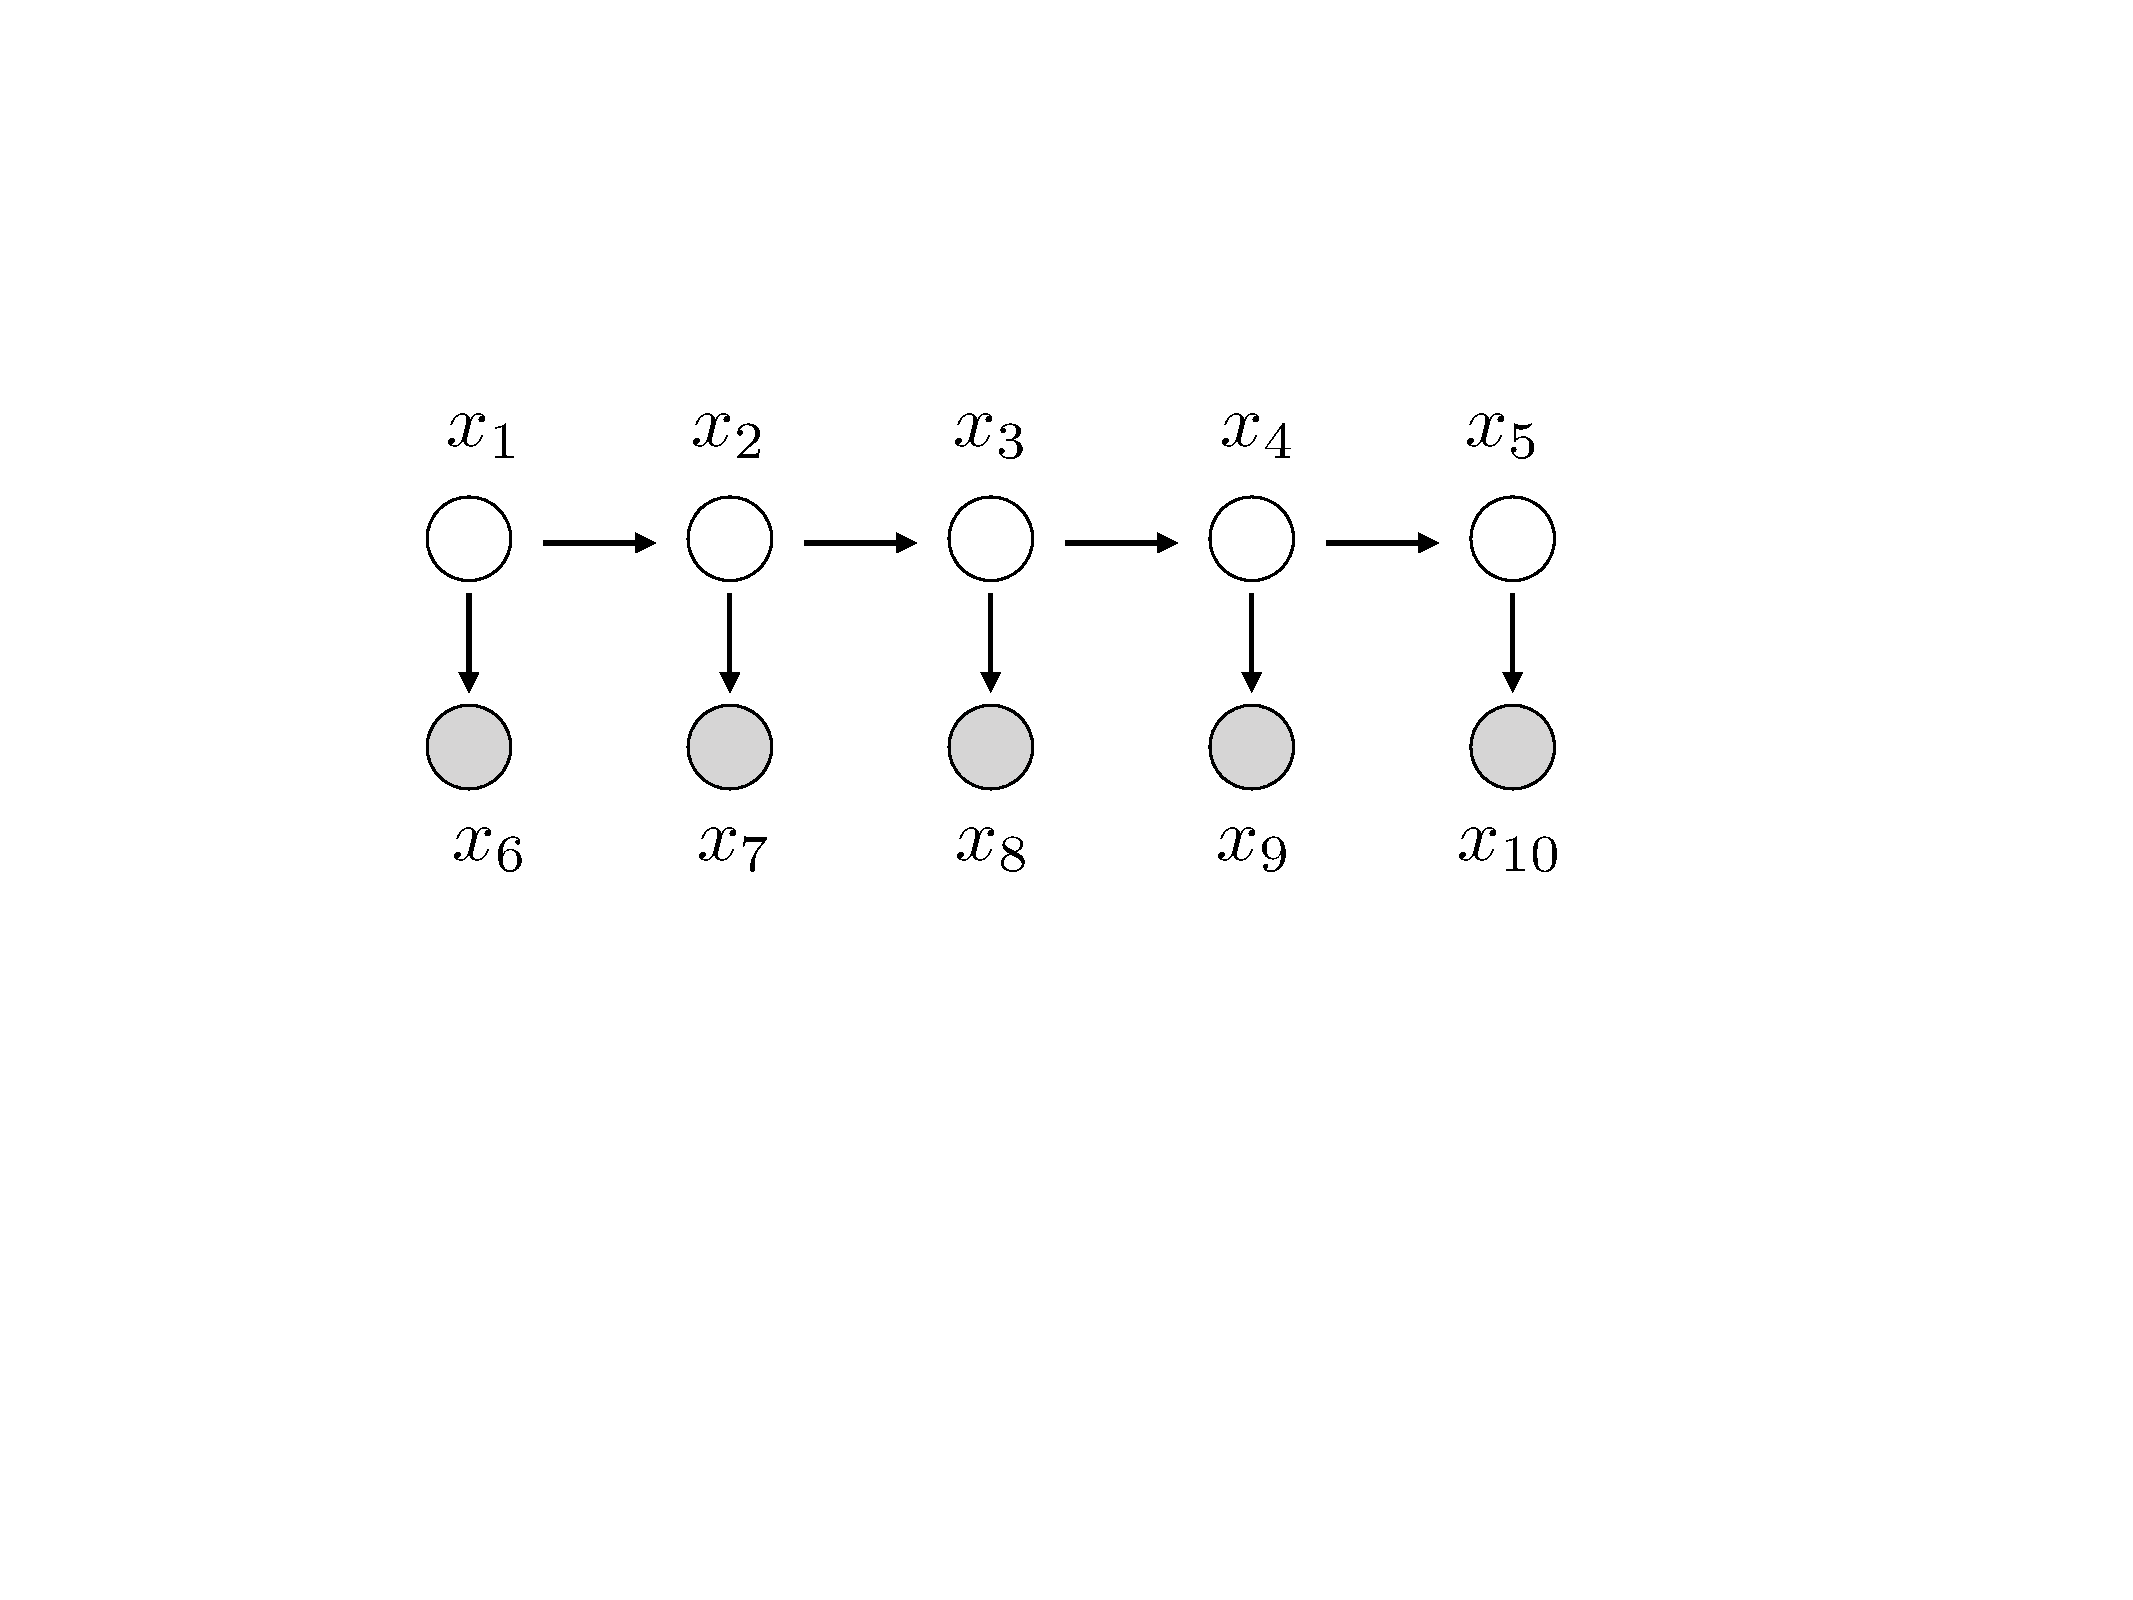
\includegraphics[width=4.5in]{gmhw1.pdf}
\end{figure}

\noindent \emph{Solution:}\\
Factorization: 
\begin{equation}
p(x_{1:10}) = p(x_1) p(x_2|x_1) p(x_3|x_2)p(x_4|x_3) p(x_5|x_4)  p(x_6|x_1) p(x_7|x_2)p(x_8|x_3) p(x_9|x_4)p(x_{10}|x_5)
\end{equation}

Conditioned on $x_3$, $x_8$ becomes independent from all variables, and $x_{1},x_2,x_6,x_7$ become independent from $x_4,x_5,x_9,x_{10}$.\\

\noindent \textbf{Problem 2. }  (10pt) Consider the \emph{sample mean} of a stationary time series  $x_t$, defined as:
\begin{equation}
\hat{\mu} = \frac{1}{T} \sum_t x_t.
\end{equation}
Compute the variance of this estimate $Var[\hat{\mu}]$, as a function of $T$, and the autocovariance function $\rho(h)$.\\
\emph{Hint: The empirical mean is also a linear combination of random variables, so you can use the formula for the covariance of linear combinations of random variables from the lecture. }\\


\noindent \emph{Solution:}\\
The empirical mean is a linear combination of (in the ARMA world, gaussian) random variables:
\begin{equation}
\hat{\mu} = \frac{1}{T} \sum_t x_t.
\end{equation}
so the variance of $\hat{\mu}$ can be expressed (using the usual formula for the covariance of linear combinations of random variables from the lecture) as:
\begin{equation}
\mathrm{Var}[\hat{\mu} ]=  \mathrm{Cov}\left[ \frac{1}{T} \sum_t x_t,  \frac{1}{T} \sum_s x_s\right] = \frac{1}{T^2} \sum_{t,s} \mathrm{Cov}[x_t,x_s] = \frac{1}{T^2} \sum_{t,s}\rho(t-s)
\end{equation}
Lots of terms in that sum, but we can group them by lag, $h$, and then count the number of $(t,s)$ pairs with the same $h$, which yields:
\begin{equation}
\mathrm{Var}[\hat{\mu} ] = \frac{1}{T^2} \sum_{h=-T}^T (T-|h|)\rho(h)
\end{equation}
As a sanity check, we can see that in the case of iid data this reduces to the usual $1/T$ scaling in CLT.\\


\noindent \textbf{Problem 3. } (10pt) Confidence bounds for the autocorrelation function: 
show that the variance of the empirical ACF for white noise with variance $\sigma^2$ estimated given $T$ data points is $\frac{1}{T}$.\\
\emph{Hint: Use theorem A.7 from Shumway, and  Stoffer  (yellow book, pdf on brightspace); alternatively, you can just show it numerically by plotting empirical estimates of the ACF as a function of T. }\\

\noindent \emph{Solution:}\\
If using A.7: for any  stationary linear process, the estimate of the ACF, $\boldsymbol{\hat{\rho}}$  is asymptotically normal, with mean $\boldsymbol{\rho}$ and covariance $\mathbf{W}$, with elements (A.54):
\begin{equation}
W_{pq} = \frac{1}{T}\sum_u \left[ \rho(u+p) +\rho(u-p) - \rho(u)\rho(p) \right] \left[ \rho(u+q) +\rho(u-q) - \rho(u)\rho(q) \right].
\end{equation}
In the special case of white noise, we have $\rho(h) = 1$ for $h=0$ and zero otherwise;  the only way to make one of the factors above nonzero is to have $u=p$ or $u=q$, but the two conditions need to be satisfied simultaneously for the product of the two to be nonzero. Hence for white noise the  covariance becomes the rescaled identity: 
$$\mathbf{W}=\frac{1}{T} \mathbf{I}$$
The confidence bounds, typically defined as 2 $times$ std are hence $2/\sqrt{T}$.\\

\noindent The same kind of scaling can be seen numerically by varying T and for each sequence length repeatedly sampling from white noise sequences, computing the ACF for each, then the variance of this estimate pooling across draws. \\
N.B. While the proof is asymptotic, the numerics should convince us that the confidence bounds behave reasonably even when $T$ is not that large.\\


\noindent \textbf{Problem 4.} (5pt+5pt) Identify the following models as $\mathrm{ARMA}(p,q)$:
\begin{itemize}
\item $x_t = 0.8 x_{t-1} - 0.15 x_{t-2} + w_t - 0.3 w_{t-1}$
\item $x_t =  x_{t-1} - 0.5 x_{t-2} + w_t - w_{t-1}$
\end{itemize}
\emph{Note: watch out for parameter redundancy!}\\


\noindent \emph{Solution:} 
\\
We first write the expression in canonical form (AR terms left, MA terms right), 
$x_t - 0.8 x_{t-1} + 0.15 x_{t-2} = w_t - 0.3 w_{t-1}$, then identify the corresponding P,Q polynomials :
\begin{eqnarray*}
P(B) &=& 1 - 0.8 B + 0.15 B^2 = (1-0.3 B)(1-0.5B) \\
 Q(B) &=& 1- 0.3 B
\end{eqnarray*}
Since the two share a factor, we need to simply the model  to:
\begin{eqnarray*}
P(B) &=&  1-0.5B \\
 Q(B) &=& 1
\end{eqnarray*}
which translates into $x_t = 0.5x_{t-1} + w_t$; this is an AR(1) process. 
P's root is 2 > 1,  so the process is causal.\\

\noindent  Similarly, the second model $x_t - x_{t-1} + 0.5 x_{t-2} = w_t - w_{t-1}$  has corresponding polynomials
\begin{eqnarray*}
P(B) &=& 1 -  B + 0.5 B^2  \\
 Q(B) &=& 1- B
\end{eqnarray*}
These don't have common roots so the model is an ARMA(2,1); P has complex roots $1\pm i$ which are outside the unit circle, so it's a causal process. 
Q has root 1: not invertible.
\\


\noindent \textbf{Problem 5.} (10pt) Given the AR(2) process with $P(B) = (1-0.2B)(1-0.5B)$, what is $\rho(h)$? 
 Check your analytical solution against an empirical estimate obtained using the code from the lab.\\
 
\emph{Hint: Difference equations + initial conditions.}\\
\noindent \emph{Solution:}\\
Using the difference equation form of the recursion and observing that the AR polynomial has two roots $z_1=5$ and $z_2 = 2$ (making it causal), we know that the functional form for the CCF is: $\rho(h) = c_1 z_1^{-|h|} + c_2 z_2^{-|h|}$, where the two constants need to be determined from initial conditions.\footnote{So dependencies decay exponentially fast.} How do we do that? One obvious initial condition is that $\rho(0) = 1$; the second constraint takes a bit more work. First, let's write out the explicit AR form:
$$ x_t = 0.7 x_{t-1} -0.1 x_{t-2} + w_t$$
The ACF recursion equation is then:
$$ \rho(h) = 0.7 \rho(h-1) -0.1 \rho(h-2)$$
Now we take $h =1$ and take advantage of the fact that $\rho(1) =\rho(-1)$ to get the second constraint:
$$ \rho(1) = \frac{7}{11}$$
To finish up, compute the cs and validate the solution numerically (-5/11 and 16/11).


\end{document}